\documentclass[a4paper, 10pt, final, garamond]{book}
\usepackage{cours-preambule}
\graphicspath{{./figures/}}

\makeatletter
\renewcommand{\@chapapp}{Contr\^ole de connaissances}
\makeatother

\toggletrue{student}
\HideSolutionstrue

\begin{document}
\setcounter{chapter}{2}

\chapter{Électrocinétique~: ARQS et résistances}

\ifstudent{
	\begin{tikzpicture}[remember picture, overlay]
		\node[anchor=north west, align=left]
      at ([shift={(1.4cm,0)}]current page.north west)
		{\\[5pt]\Large\bfseries Nom~:\\[10pt]\Large\bfseries Prénom~:};
		\node[anchor=north east, align=right]
      at ([shift={(-1.5cm,-17pt)}]current page.north east)
		{\Large\bfseries Note~:\hspace{1cm}/10};
	\end{tikzpicture}
}

\begin{enumerate}[label=\sqenumi, leftmargin=10pt]
	\nitem{2} Donner les quatre propriétés de la charge électrique.
  \smallbreak
  \wsw{
    $Q$ est algébrique ($\lessgtr 0$), additive ($Q = \sum_i q_i$), quantifiée
    ($Q = k \times e$ avec $k \in \Zb$), et $Q$ est conservée si le système est
    isolé.
  }
	% \nitem{2} Réprésenter deux dipôles en série avec toutes les tensions et
	% intensités, fléchées en convention récepteur. Quelle caractéristique des
	% dipôles en série partagent-ils~? Même question pour des dipôles en parallèle.
	% \begin{isd}
	%   \tcbsubtitle{\fatbox{En série}}
	%   \begin{center}
	%     \switch{
	%             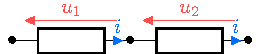
\includegraphics[width=\linewidth, draft=true]{serie_rec}
	%     }{
	%     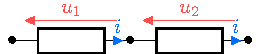
\includegraphics[width=\linewidth]{serie_rec}
	%     }
	%   \end{center}
	%   Deux dipôles en série partagent la même intensité.
	%   \tcblower
	%   \tcbsubtitle{\fatbox{En parallèle}}
	%   \begin{center}
	%     \switch{
	%             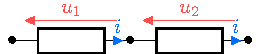
\includegraphics[width=\linewidth, draft=true]{serie_rec}
	%     }{
	%     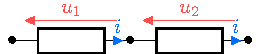
\includegraphics[width=\linewidth]{serie_rec}
	%     }
	%   \end{center}
	%   Deux dipôles en série partagent la même intensité.
	% \end{isd}
	\nitem{2}
  \begin{minipage}[t]{0.50\linewidth}
    % \vspace{5cm}
		Pour le circuit ci-contre, établir les liens entre les différents
		courants et les différentes tensions.
    \begin{center}
      \switch{
        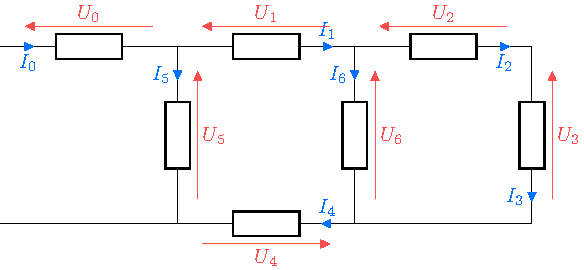
\includegraphics[width=\linewidth]{exer_ldnm_plain}
      }{
        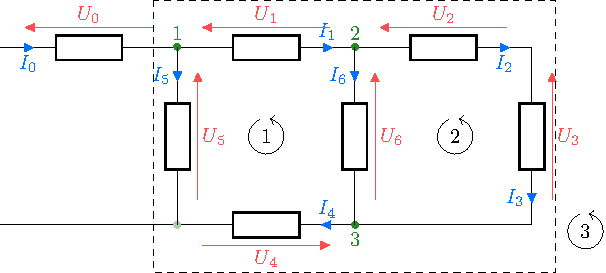
\includegraphics[width=\linewidth]{exer_ldnm}
      }
      \captionof{figure}{}
    \end{center}
	\end{minipage}
  \hfill
  \begin{minipage}[t]{.5\linewidth}
    ~
    \vspace{-20pt}
      \begin{tcolorbox}[blankest]
        \begin{center}
          \fbox{Lois des nœuds}
        \end{center}
        \vspace{-15pt}
      \wsw{
        \begin{itemize}
          \item $I_2 = I_3$ par unicité à droite ;
          \item $I_0 = I_1 + I_5$ par LdN 1 ;
          \item $I_1 = I_2 + I_6$ par LdN 2 ;
          \item $I_3 + I_6 = I_4$ par LdN 3.
        \end{itemize}
      }
      \tcblower
        \begin{center}
          \fbox{Lois des mailles}
        \end{center}
        \vspace{-15pt}
      \wsw{
        \begin{itemize}
          \item $U_4 + U_6 + U_1 = U_5$ par LdM 1 ;
          \item $U_3 + U_2 = U_6$ par LdM 2 ;
        \end{itemize}
      }
    \end{tcolorbox}
  \end{minipage}
  \nitem{2} Représenter deux résistances $R_1$ et $R_2$ en série. Démontrer
  l'expression $R_{\rm eq}$ de la résistance équivalente à $R_1$ et $R_2$.
  \begin{isd}[lefthand ratio=.3]
		\begin{center}
			\switch{
				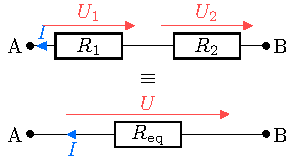
\includegraphics[width=\linewidth, draft=true]{rserie}
			}{
				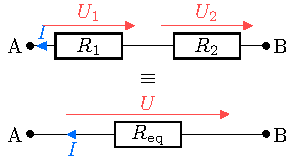
\includegraphics[width=\linewidth]{rserie}
			}
      \captionof{figure}{}
		\end{center}
    \tcblower
    \wsw{
          Comme elles sont en série, elles partagent $I$.
          \begin{align*}
            U & = U_1 + U_2    \\
            U & = R_1I + R_2I  \\
            U & = (R_1 + R_2)I
          \end{align*}
          D'où $R_{\rm eq} = R_1+R_2$.
    }
  \end{isd}
  \nitem{2} Représenter deux résistances $R_1$ et $R_2$ en parallèle. Démontrer
  l'expression $R_{\rm eq}$ de la résistance équivalente à $R_1$ et $R_2$.
  \begin{isd}[lefthand ratio=.3]
		\begin{center}
			\switch{
				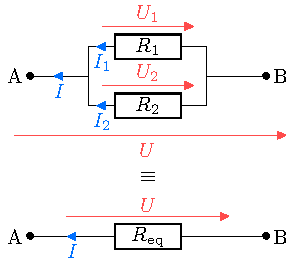
\includegraphics[width=.5\linewidth, draft=true]{rpara}
			}{
				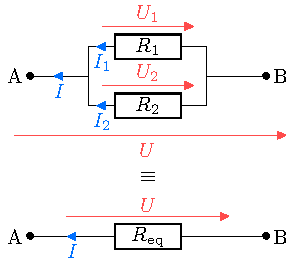
\includegraphics[width=.5\linewidth]{rpara}
			}
      \captionof{figure}{}
		\end{center}
    \tcblower
		\wsw{
    Comme elles sont en parallèle, elles partagent $U$.
      \begin{DispWithArrows*}[]
        I &= I_1 + I_2
        \Arrow{$I = GU$}
        \\\Lra
        G_{\rm eq}U &= (G_1+G_2)U
        \\\Lra
        R_{\rm eq} &= \frac{R_1R_2}{R_1+R_2}
      \end{DispWithArrows*}
		}
  \end{isd}
  \nitem{2} Donner et démontrer la relation du pont diviseur de tension pour
  deux résistances $R_1$ et $R_2$ en série.\\
  \begin{isd}[lefthand ratio=.15]
		\begin{center}
			\switch{
				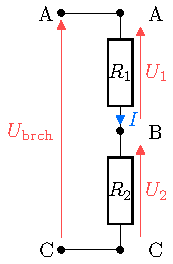
\includegraphics[width=\linewidth, draft=true]{divis_tension}
			}{
				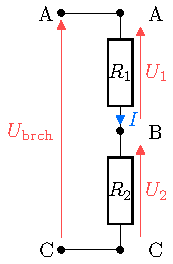
\includegraphics[width=\linewidth]{divis_tension}
			}
      \captionof{figure}{}
  \vspace*{-15pt}
		\end{center}
    \tcblower
		\wsw{
		Avec une loi des mailles et la loi d'Ohm pour les résistances, on trouve
		\[
			I = \frac{U_{\rm brch}}{R_1+R_2}
		\]
		En réappliquant la loi d'Ohm pour $R_k$, on trouve
		\[
			U_{k} = R_kI = \frac{R_k}{R_1+R_2}U_{\rm brch}
		\]
		}
	\end{isd}
  \vspace*{-15pt}
\end{enumerate}
\end{document}
